\documentclass{article}

\usepackage[a4paper, total={7in, 10in}]{geometry}

\usepackage{hyperref}
\usepackage{amsmath}
\usepackage{subcaption}
\usepackage{graphicx}
\graphicspath{{../Results/Protected/}}

\title{AIMS Course 1: Data, Estimation and Inference}
\author{Jake Levi}
\date{October 2022}

\begin{document}
\maketitle

% Section: introduction

\section{Introduction}

This lab report investigates the use of Gaussian Processes (GPs), a type of machine learning model motivated by Bayesian probability theory, for modelling a meteorological dataset called Sotonmet. In a GP model, given a mean function $\mu$, kernel function $K$, vaiance of observation noise $\sigma^2$, training inputs $x$ (represented as a vector), and prediction inputs $x^*$, the noisy training labels $y$ (which we assume are noisy observations of unknown labels $f$) and noiseless prediction labels $f^*$ have a joint Gaussian distribution:

% Equation: joint distribution

\begin{equation}
    p\left( \begin{bmatrix}
        y \\
        f^*
    \end{bmatrix} \right)
    = \mathcal{N} \left( \begin{bmatrix}
        y \\
        f^*
    \end{bmatrix} \middle| \begin{bmatrix}
        \mu(x) \\
        \mu(x^*)
    \end{bmatrix}, \begin{bmatrix}
        K(x, x) + \sigma^2 I & K(x, x^*) \\
        K(x, x^*)^T & K(x^*, x^*) \\
    \end{bmatrix} \right)
\end{equation}

Where $K(x, x^*)$ is a matrix whose $(i, j)$th element is given by $K(x, x^*)_{i,j} = K(x_i, x^*_j)$. The predictive distribution $p(f^* \mid y)$ follows from the formula for the conditional distribution of a jointly Gaussian random variable \cite{bishop2006pattern}:

% Equation: conditional distribution

\begin{align}
    p(f^* \mid y) &= \mathcal{N}\left(f^* \mid \mu^*, \Sigma^* \right) \\
    \text{where} \quad \mu^* &= \mu(x^*) + K(x^*, x) \left( K(x, x) + \sigma^2 I \right)^{-1} (y - \mu(x)) \\
    \Sigma^* &= K(x^*, x^*) - K(x^*, x) \left( K(x, x) + \sigma^2 I \right) ^{-1} K(x, x^*)
\end{align}

The log marginal likelihood (LML) of the noisy training labels $y$ given training input data $x$ (and also implicitly given any hyperparameters of the model) is given by:

% Equation: log marginal likelihood

\begin{align}
    \log \left( p(y \mid x) \right) &= -\frac{1}{2}\log\left(\det \left(2\pi \Sigma_y \right)\right) -\frac{1}{2}(y - \mu(x))^T \Sigma_y^{-1} (y - \mu(x)) \\
    \text{where} \quad \Sigma_y &= K(x, x) + \sigma^2 I
\end{align}

This expression implies that maximising the LML encourages $\mu(x)$, $K(x,x)$ and $\sigma$ to fit the data accurately and with calibrated uncertainty. Maximising the LML can also be motivated from a Bayesian perspective, which is discussed further in Appendix \ref{appendix:why_lml}.

The focus in this coursework submission is on predicting the tide height given the time of day, for which the training and ground truth data is shown in Figure \ref{fig:data}, alongside an independent GP prediction in Figure \ref{fig:ind_pres}.

% Section: results

\section{Results}

We start off by considering GPs with constant mean function and squared exponential kernel, whose mean and kernel functions are related to the hyperparameters $c$, $k$, and $\lambda$ as follows ($\sigma$ is also considered to be a hyperparameter, although it is not explicitly part of the mean or kernel functions):

% Equation: constant mean and squared exponential kernel function

\begin{align}
\mu(x) &= c \\
K_{\mathrm{sqe}}(x, x') &= k \exp\left( -\left( \frac{x - x'}{\lambda} \right)^2 \right)
\end{align}

Within the domain of such GPs, we start off by considering two GPs denoted by sqe\_1 and sqe\_2, as described in Table \ref{table:sqe_details_table}. Samples from the prior distributions of sqe\_1 and sqe\_1 are shown in Figures \ref{fig:prior_sqe_1} and \ref{fig:prior_sqe_2}, which show that the prior distribution of sqe\_1 looks subjectively like a much more plausible explanation for the data. The predictive distributions of these GPs are shown in Figures \ref{fig:pred_dist_sqe_1} and \ref{fig:pred_dist_sqe_2}, which show that, although sqe\_1 produced a \emph{prior} distribution which looks like a more plausible explanation for the training data, sqe\_2 produces a \emph{predictive} distribution which looks like a much better fit to the training data. Furthermore, the predictive distribution of sqe\_1 is "confidently wrong" (the mean is far away from the ground truth labels and with high certainty/low standard deviation) in regions containing ground truth labels but no training data, which could be a very undesirable property in a safety-critical prediction scenario. Samples from the predictive distribution of both GPs are shown in Figures \ref{fig:pred_samples_sqe_1} and \ref{fig:pred_samples_sqe_2}, which show that neither GP produces samples that reflect the data distribution particularly well.

Metrics, hyperparameter optimisation, etc. Remarkably, sqe\_opt has worse RMSE on train data than sqe\_1, but better RMSE on ground truth data, which implies that maximising the log marginal likelihood alone encourages models not to overfit their training data, and furthermore to generalise well to unseen data, which arguably is the entire purpose of supervised machine learning.

\appendix

% Figure: Sotonmet dataset

\begin{figure}[pht]
    \centering
    \subfloat[
        \centering Training and ground truth data
        \label{fig:data}
    ]{
        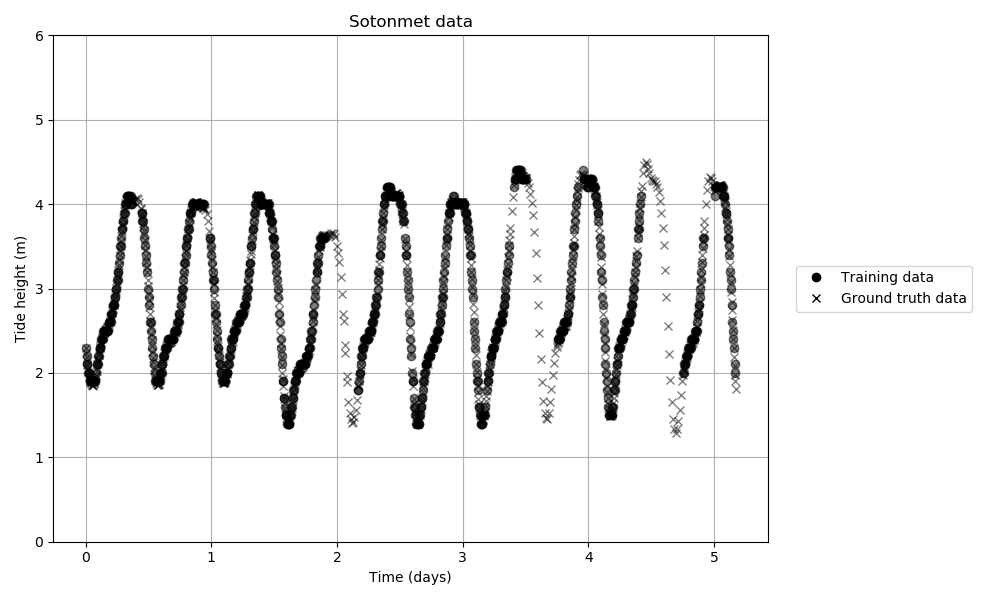
\includegraphics[width=0.45\textwidth]{Sotonmet_data.png}
    }
    \subfloat[
        \centering Independent GP predictions
        \label{fig:ind_pres}
    ]{
        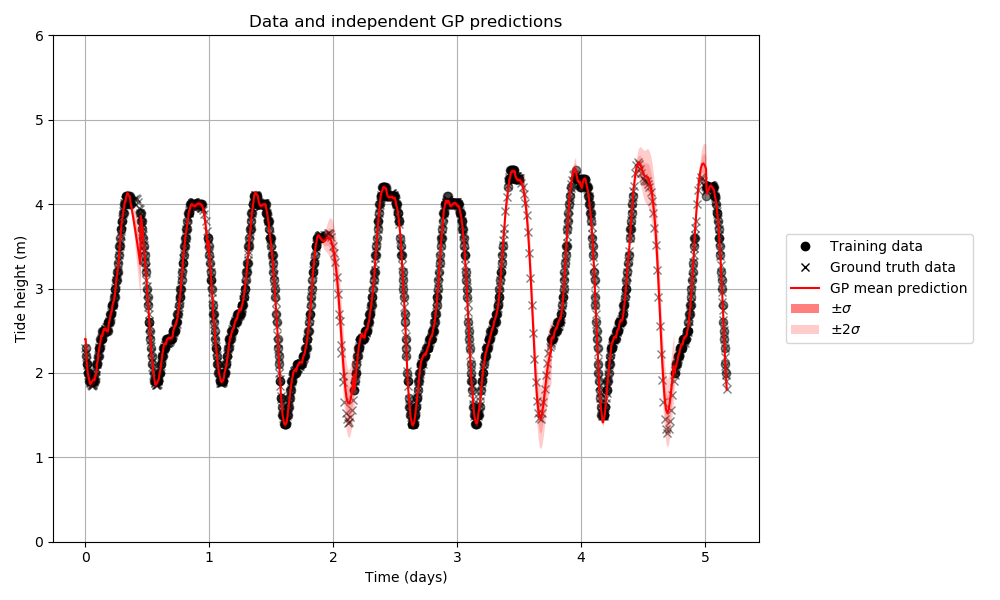
\includegraphics[width=0.45\textwidth]{Data_and_independent_GP_predictions.png}
    }
    \caption{The Sotonmet dataset}
    \label{fig:sotonmet}
\end{figure}

% Figure: GPs with SQE kernel

\begin{figure}[pht]
    \centering
    \begin{subfigure}{0.45\textwidth}
        \centering
        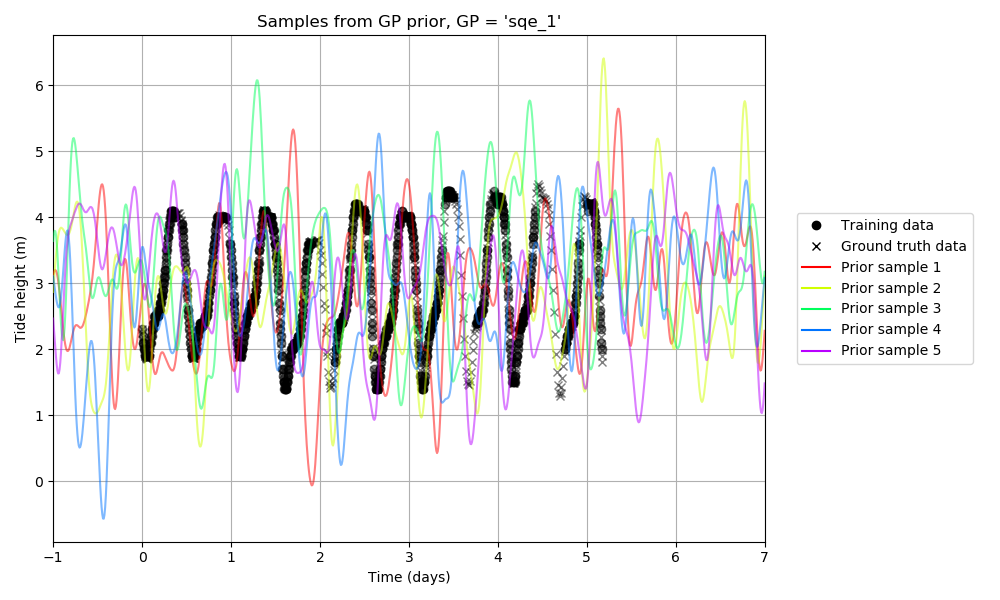
\includegraphics[width=\textwidth]{Samples_from_GP_prior,_GP____sqe_1_.png}
        \caption{Samples from the prior of sqe\_1}
        \label{fig:prior_sqe_1}
    \end{subfigure}
    \begin{subfigure}{0.45\textwidth}
        \centering
        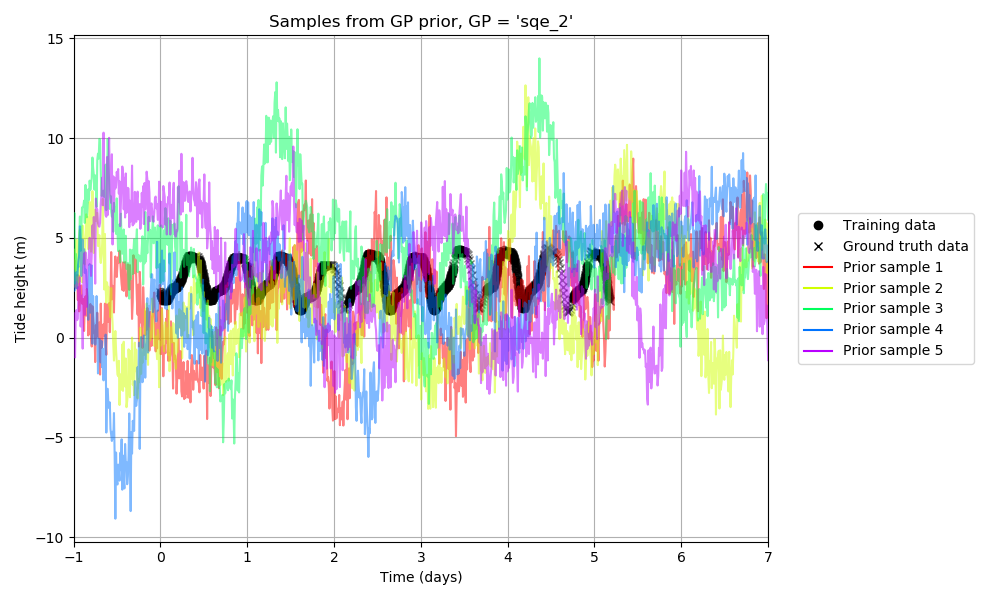
\includegraphics[width=\textwidth]{Samples_from_GP_prior,_GP____sqe_2_.png}
        \caption{Samples from the prior of sqe\_2}
        \label{fig:prior_sqe_2}
    \end{subfigure}
    \newline
    \begin{subfigure}{0.45\textwidth}
        \centering
        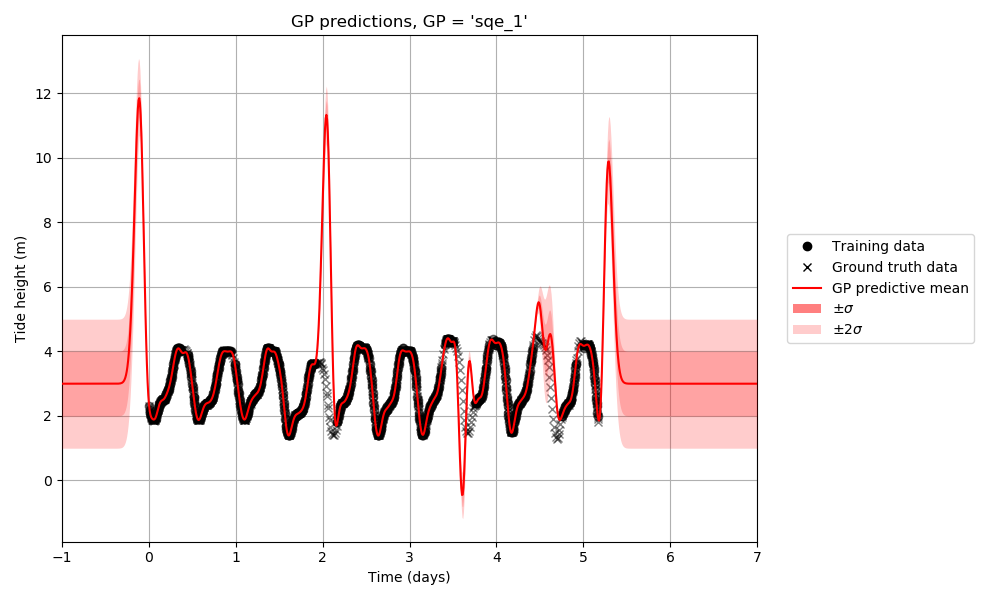
\includegraphics[width=\textwidth]{GP_predictions,_GP____sqe_1_.png}
        \caption{Predictive distribution of sqe\_1}
        \label{fig:pred_dist_sqe_1}
    \end{subfigure}
    \begin{subfigure}{0.45\textwidth}
        \centering
        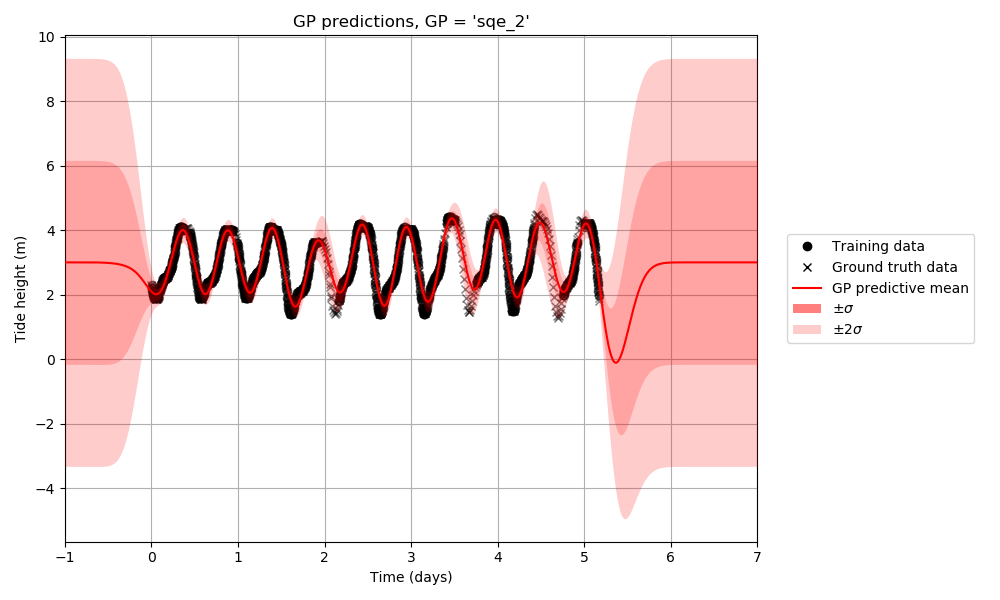
\includegraphics[width=\textwidth]{GP_predictions,_GP____sqe_2_.png}
        \caption{Predictive distribution of sqe\_2}
        \label{fig:pred_dist_sqe_2}
    \end{subfigure}
    \newline
    \begin{subfigure}{0.45\textwidth}
        \centering
        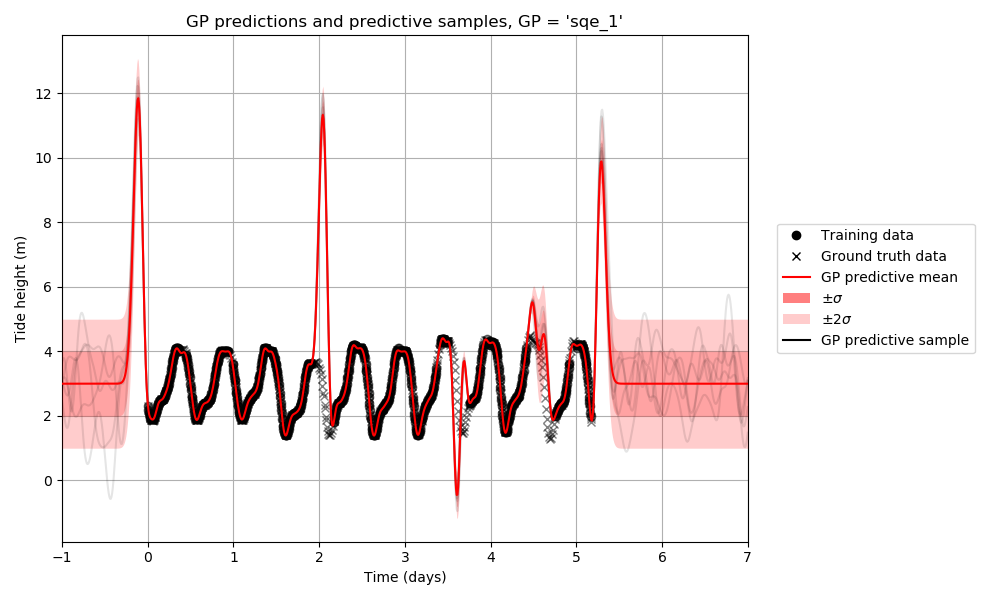
\includegraphics[width=\textwidth]{GP_predictions_and_predictive_samples,_GP____sqe_1_.png}
        \caption{Samples from the predictive distribution of sqe\_1}
        \label{fig:pred_samples_sqe_1}
    \end{subfigure}
    \begin{subfigure}{0.45\textwidth}
        \centering
        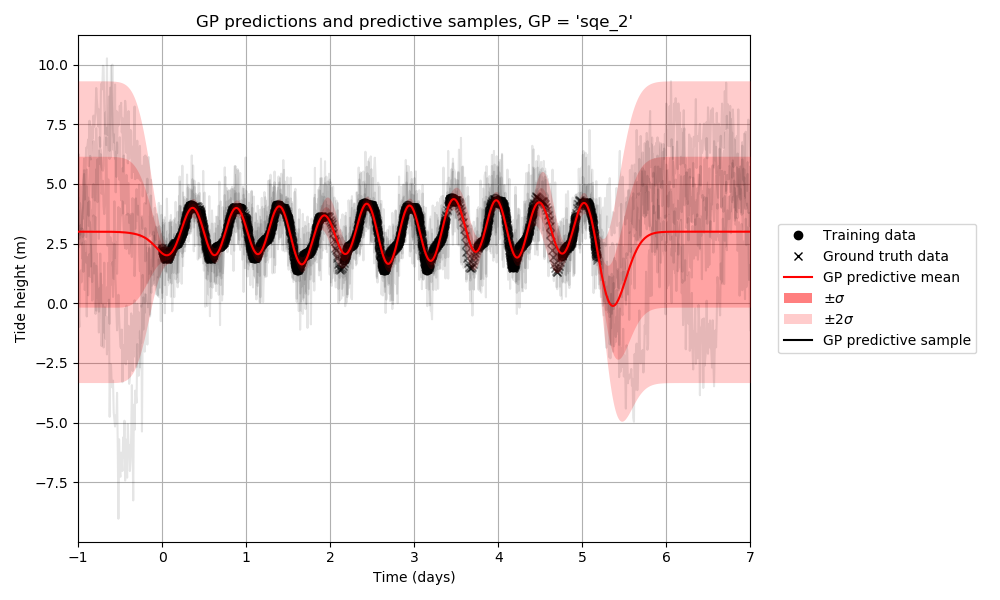
\includegraphics[width=\textwidth]{GP_predictions_and_predictive_samples,_GP____sqe_2_.png}
        \caption{Samples from the predictive distribution of sqe\_2}
        \label{fig:pred_samples_sqe_2}
    \end{subfigure}

    \caption{Prior and predictive distributions of GPs with square exponential kernels}
    \label{fig:sqe}
\end{figure}

% Table: SQE GPs

\begin{table}[ht]
    \centering
    \begin{tabular}{|c|c|c|c|}
        \hline
        Hyperparameter & sqe\_1 & sqe\_2 & sqe\_opt \\
        \hline
        $c$ & 3.0000 & 3.0000 & 2.9905 \\
        $\lambda$ & 0.1000 & 0.3000 & 0.0867 \\
        $k$ & 1.0000 & 10.0000 & 0.6522 \\
        $\sigma$ & 0.0010 & 1.0000 & 0.0293 \\
        \hline
    \end{tabular}
    \caption{Description of GPs with squared exponential kernel that were evaluated in this report}
    \label{table:sqe_details_table}
\end{table}

% Table: SQE metrics

\begin{table}[ht]
    \centering
    \begin{tabular}{|c|c|c|c|}
        \hline
        Metric & sqe\_1 & sqe\_2 & sqe\_opt \\
        \hline
        RMSE (train) & 0.0268 & 0.2246 & 0.0275 \\
        RMSE (truth) & 0.8040 & 0.2573 & 0.1587 \\
        LML & -327743.8 & -942.0 & 1574.4 \\
        LPL (train) & -321611.9 & -875.4 & 1954.9 \\
        LPL (truth) & -87596.3 & -894.3 & 3366.3 \\
        \hline
    \end{tabular}
    \caption{Metrics used to evaluate GPs with squared exponential kernels}
    \label{table:sqe_metrics_table}
\end{table}

\section{Motivation for maximising the log marginal likelihood}\label{appendix:why_lml}

% References and end of document

\bibliographystyle{plain}
\bibliography{references}

\end{document}
